
%----------------------------------------------------------------------------------------
%	PACKAGES AND OTHER DOCUMENT CONFIGURATIONS
%----------------------------------------------------------------------------------------
\pdfoutput=1
\documentclass[fleqn,10pt]{SelfArx} % Document font size and equations flushed left

\usepackage[english]{babel} % Specify a different language here - english by default

\usepackage[super,biblabel]{cite} % Superscript citations

\usepackage{setspace} % for block quoting

\usepackage{etoolbox}

\usepackage{graphicx}

\usepackage{listings}

\usepackage[htt]{hyphenat}

\usepackage{graphicx}

\usepackage{algpseudocode}

\lstdefinestyle{mystyle}{basicstyle=\ttfamily\footnotesize}
\lstset{style=mystyle}

\AtBeginEnvironment{quote}{\singlespace\vspace{-\topsep}\small}
\AtEndEnvironment{quote}{\vspace{-\topsep}\endsinglespace}

\graphicspath{ {figures/} }


%----------------------------------------------------------------------------------------
%	COLUMNS
%----------------------------------------------------------------------------------------

\setlength{\columnsep}{0.55cm} % Distance between the two columns of text
\setlength{\fboxrule}{0.75pt} % Width of the border around the abstract

%----------------------------------------------------------------------------------------
%	COLORS
%----------------------------------------------------------------------------------------

\definecolor{color1}{RGB}{0,0,90} % Color of the article title and sections
\definecolor{color2}{RGB}{0,20,20} % Color of the boxes behind the abstract and headings

%----------------------------------------------------------------------------------------
%	HYPERLINKS
%----------------------------------------------------------------------------------------

\usepackage{hyperref} % Required for hyperlinks
\hypersetup{hidelinks,colorlinks,breaklinks=true,urlcolor=color2,citecolor=color1,linkcolor=color1,bookmarksopen=false,pdftitle={Title},pdfauthor={Author}}

%----------------------------------------------------------------------------------------
%	ARTICLE INFORMATION
%----------------------------------------------------------------------------------------

% \JournalInfo{..., 2020} % Journal information
% \Archive{arXiv pre-print} % Additional notes (e.g. copyright, DOI, review/research article)

\PaperTitle{JAMPI: efficient matrix multiplication in Spark using Barrier Execution Mode} % Article title

\Authors{Tamas Foldi\textsuperscript{1}*, Chris von Csefalvay\textsuperscript{1}, Nicolas A Perez\textsuperscript{2}} % Authors
\affiliation{\textsuperscript{1}\textit{Starschema Inc., Arlington, VA.}} % Author affiliation
\affiliation{\textsuperscript{1}\textit{Hewlett Packard Enterprise,  Miami, FL.}} % Author affiliation
\affiliation{*\textbf{Corresponding author}: tfoldi@starschema.net} % Corresponding author

% \Keywords{Spark --- Matrix multiplication --- Algorithmic methods} % Keywords - if you don't want any simply remove all the text between the curly brackets
% \newcommand{\keywordname}{Keywords} % Defines the keywords heading name

%----------------------------------------------------------------------------------------
%	ABSTRACT
%----------------------------------------------------------------------------------------

\Abstract{The new barrier mode in Apache Spark allows embedding distributed deep learning training as a Spark stage to simplify the distributed training workflow. In Spark, a task in a stage doesn’t depend on any other tasks in the same stage, and hence it can be scheduled independently. However, several algorithms require more sophisticated inter-task communications, similar to the MPI paradigm. By combining distributed message passing (using asynchronous network io), OpenJDK's new autovectorization and Spark's barrier mode, we can add non-map/reduce based algorithms, such as Cannon's distributed matrix multiplication, improving the performance of the existing MLlib implementation. This paper discloses an efficient distributed matrix multiplication algorithm within a barrier task, which results in an XXX\% performance increase on a 10,000x10,000 square matrix with XXX\% less memory footprint. Applications of efficient matrix multiplication include significantly accelerating the training and implementation of deep convolutional neural network based workloads.}

%----------------------------------------------------------------------------------------

\begin{document}
%\flushbottom % Makes all text pages the same height
\maketitle % Print the title and abstract box
%\tableofcontents % Print the contents section
% \thispagestyle{empty} % Removes page numbering from the first page

%----------------------------------------------------------------------------------------
%	ARTICLE CONTENTS
%----------------------------------------------------------------------------------------

\section{Introduction} % (fold)
\label{sec:introduction}

The recent decade has seen the emergence of two immensely powerful processes in tandem: the rise of big data handling solutions like Apache Spark on one hand and the apotheosis of deep learning as the tool of choice for demanding computational solutions for machine learning problems. Yet at its essence, big data and deep learning remain not only separate communities but also significantly separate domains of software. Despite deep learning over big data becoming a crucial tool in a range of applications, including in computer vision,\cite{guo2016deep,voulodimos2018deep}  bioinformatics,\cite{spencer2014deep,alipanahi2015predicting,zhang2016deep,wei2018prediction} natural language processing (NLP),\cite{deselaers2009deep,socher2012deep,young2018recent,otter2020survey} clinical medicine,\cite{bar2015chest,havaei2016deep,liu2017detecting,stead2018clinical,campanella2019clinical,lehman2019mammographic} anomaly detection in cybersecurity and fraud detection,\cite{du2017deeplog,shone2018deep,chalapathy2019deep} and collaborative intelligence/recommender systems,\cite{wang2015collaborative,deng2016deep,karatzoglou2017deep,batmaz2019review} its full potential remains to be harnessed. The primary impediment in this respect is largely a divergence of attitudes and concerns, leading to two divergent paradigms of development:

\begin{itemize}
	\item \emph{The big data paradigm}, primarily designed around RDDs and the the DataFrame-based API. This outlook has dominated the development of Apache Spark.
	\item \emph{The DL/ML paradigm}, which is primarily focused on efficient linear algebra operations to facilitate machine learning approaches, especially matrix algebra for deep neural networks.
\end{itemize}

The future of deep learning over big data depends greatly on facilitating the convergence of these two worlds into a single, unified paradigm: the use of well-designed big data management tools, such as Apache Spark, to interoperate with the demands of deep learning. The road towards this convergence depends on the development of efficient matrix primitives that facilitate rapid calculations over distributed networks and large data sets.

\begin{figure}
	\centering
	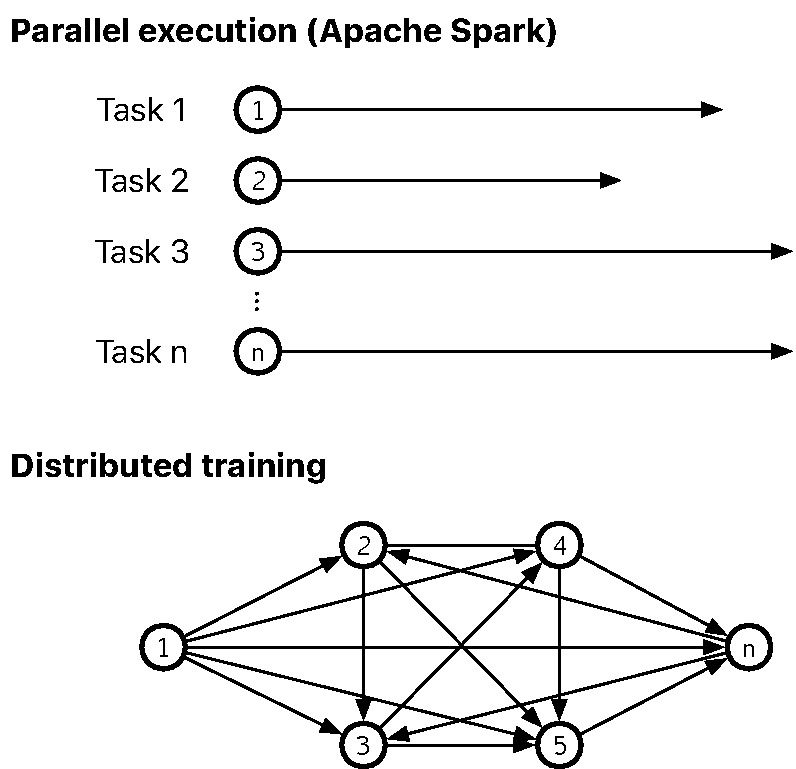
\includegraphics[width=0.9\linewidth]{figures/fig1.pdf}
	\vspace{14pt}
	\caption{Comparative execution models: Apache Spark versus distributed training for neural networks.}
	\label{fig:execution-models}
\end{figure}

The current execution model of Apache Spark is principally focused on independent, embarrassingly parallel tasks that are run and scaled, but the needs of deep learning are primarily focused on distributed training: the performance of completely communicating and coordinating tasks, optimised for interconnectivity rather than independent parallel running, while also maintaining scalability and efficiency. With the recent introduction of the barrier execution mode in Apache Spark, it has finally become possible to construct a computational approach that allows for such networked execution to take place, facilitating distributed training of deep neural networks (see Figure~\ref{fig:execution-models}).

JAMPI (Java Assisted Matrix Product with Inter-task communication), the framework described in this paper, is an efficient and rapid solution to an aspect of efficienty matrix primitives, namely matrix multiplication. By integrating JDK's new \texttt{Vector API}, asynchronous network IO (\texttt{nio}) for distributed message passing and Spark's barrier mode, a pure Scala implementation of Cannon's 2.5D matrix multiplication algorithm can be devised that is significantly more efficient than \texttt{MLlib}'s \texttt{BlockMatrix.multiply} function. JAMPI thus avoids reliance on foriegn, low level or native code in combination with \texttt{JNI} on one hand, being a pure Scala implementation. On the other hand, it provides a pre-written framework that integrates with Spark as a native task rather than an external MPI procedure call, and handles inter-task communication directly, yielding performance benefits that would otherwise be associated with a low-level MPI implemented resource negotiation framework.

\subsection{Cannon's algorithm} % (fold)
\label{sub:cannon_s_algorithm}

Matrix multiplication plays a significant role in a range of practical applications, including (but not limited to) scientific computing, non-linear modelling, agent-based models and the training of deep convolutional neural networks (deep learning). The proliferation of deep learning as the cognitive technology of choice for problems with large source data sets and high-dimensional or high-order multivariate data means that efficiency gains in the underlying linear algebra primitives has the potential to enable significant performance benefits in a wide range of use cases. In particular, constructing primitives that leverage computational capacity through rapid parallel computation and efficient interchange lends itself as an avenue towards these performance gains. While packages comprising efficient matrix primitives already exist,\cite{chetlur2014cudnn} these often operate at a low level and do not integrate well with existing and proven solutions to manage large computational loads.


The matrix multiplication operation $\star$ for an $p \times q$ matrix $\mathbf{A}$ and an $q \times r$ matrix $B$ is defined so that for the resultant matrix $\mathbf{C} = \mathbf{A} \star \mathbf{B}$, each element $c_{i, j}$ is the dot product of the $i$-th row of $\mathbf{A}$ and the $j$-th row of $\mathbf{B}$, i.e.

$$ c_{i, j} = \sum_{k = 1}^n a_{i, k} b_{k, j} $$

The multiplication of square matrices constituites a special case. For a square matrix of order $n$, i.e. an $n \times n$ matrix, a special case obtains, which can be resolved efficiently using Cannon's algorithm.\cite{cannon1969cellular} 

For a square matrix of order $n$, i.e. $n \times n$, Cannon's algorithm uses a toroidally connected mesh $\mathbf{P}^{n \times n}$ of $n^2$ processes. Rendered in pseudocode, the algorithm can be expressed as follows for $p$ processors:

\begin{algorithmic}
	\ForAll{i = 0 : $\sqrt{p}$ - 1}
		\State CShift left A[i; :] by i 
	\EndFor
	
	\ForAll{j = 0 : $\sqrt{p}$ - 1}
		\State CShift up B[:; j] by j 
	\EndFor
	
	\For{k = 0 : $\sqrt{p}$ - 1}
		\For{i = 0 : $\sqrt{p}$ - 1, j = 0 : $\sqrt{p}$ - 1}
			\State C[i, j] += A[i, j] * B[i, j]
			\State CShift left A[i; :] by 1
			\State CShift up B[:; j] by 1
		\EndFor
	\EndFor
\end{algorithmic}

Cannon's algorithm is designed to be performed on a virtual square grid $\mathbf{P}$ of $p$ processors (i.e. a $\sqrt{p} \times \sqrt{p}$ matrix). The multiplicand and multiplier matrices $\mathbf{A}$ and $\mathbf{B}$ are laid out on $\mathbf{P}$, after which the $i$-th row of $\mathbf{A}$ is circularly shifted by $i$ to the left and the $j$-th column of $\mathbf{B}$ circularly shifted by $j$ elements up. Then, $n$ times, the two entries mapped onto $p_{i, j}$ are multiplied and added onto the running value of $p_{i, j}$, after which each row of $\mathbf{A}$ is shifted left by one element and each column of $\mathbf{B}$ is shifted up by one element.

Standard methods of multiplying dense matrices require $O(n^3)$ floating operations for an $n \times n$ matrix. Cannon's algorithm improves on this by reducing it to $O(\frac{n^3}{p})$. In particular, because of the fact that memory is not dependent on the number of processors, it scales dynamically with the number of processors. This makes it an attractive candidate for implementation as a high-performance distributed matrix multiplication primitive.

% subsection cannon_s_algorithm (end)

\subsection{Spark's barrier mode} % (fold)
\label{sub:spark_s_barrier_mode}

Spark's barrier mode is a new mode of execution introduced to Apache Spark as part of Project Hydrogen.\cite{projecthydrogensite} Barrier execution features gang scheduling on top of the MapReduce execution model to support distributed deep learning tasks that are executed or embedded as Spark steps. The current implementation ensures that all tasks (limited to \texttt{mapPartitions}) are executed at the same time, and collectively cancels and restarts all tasks in case of failure events. In addition to true parallel execution, the workers' host names and partition identifiers are accessible inside the tasks, alongside a \texttt{barrier} call, similar to MPI's \texttt{MPI\_Barrier} function.\cite{projecthydrogenpres}

While this functionality is sufficient to support the primary use case of Spark's barrier mode -- namely, executing embedded MPI or other foreign, i.e. non-Spark and non-JVM, steps within a Spark application --, it does not provide any inter-task communication primitive to implement the same algoritms within JVM/Spark native steps. In fact, the design documentation for Spark's barrier mode clearly defines this as outside the scope of the project, stating that beyond a simple \texttt{BarrierTaskContext.barrier()} call, no intra-communication functionality will be part of the implementation. It is assumed that such functionality would be handled by the user program. It is our view based on our extensive experience with implementing deep learning solutions on distributed systems that this is a clear show-stopper: if Spark is to be a force to be reckoned with as the data layer for deep learning applications over big data, it should not force execution outside Spark's boundaries.

% subsection spark_s_barrier_mode (end)

% section introduction (end)

\section{Methods} % (fold)
\label{sec:methods}

\subsection{Cannon's algorithm on MPI} % (fold)
\label{sub:cannon_s_algorithm_on_mpi}

The MPI version of the algorithm described in Subsection~\ref{sub:cannon_s_algorithm} relies on MPI's Cartesian topology. After setting up a 2D communication grid of processors with \texttt{MPI\_Cart\_create}, processors exchange data with their neighbors by calling \texttt{MPI\_Sendrecv\_replace}. In the main loop, each processor executes a local dot product calculation, then shifts the results horizontally for matrix \texttt{a} and vertically for matrix \texttt{b}. In our benchmarks, we used \texttt{MPICH} version 3.3.2 as the underlying MPI implementation.

To speed up matrix multiplication, we applied \texttt{-O4} \texttt{-ftree-vectorize} \texttt{-march=native} GNU C compiler flags to ensure vectorized code execution. By vectorization, we refer using SIMD (Single Instruction, Multiple Data) CPU features, more precisly Advanced Vector Extensions (AVX-512F) that allows faster execution of fused multiply–add (\texttt{{FMAC}}) operations in local/partial matrix dot product steps. After compilating our code with GCC 7.3.1 we ensured that the disassembed code contains \texttt{vfmadd231sd} instruction for vectorized \texttt{FMAC}. 

% subsection cannon_s_algorithm_on_mpi (end)

\subsection{JAMPI} % (fold)
\label{sub:jampi_implementation}

JAMPI is a \emph{de novo} native Scala implementation of Cannon's algorithm as described in described in Subsection~\ref{sub:cannon_s_algorithm}. For message passing, we built an \texttt{nio} based asynchronous message passing library that mimics MPI's Cartesian topology and send-receive-replace functionality. To avoid unnecessary memory copies and to optimize performance for both throughput and latency, our \texttt{PeerMessage} object allocates fixed 8MB off-heap buffers for both sending and receiving data. Send and receive network operations are executed asynchronously and in parallel.

The matrix multiplication is embedded into a barrier execution task, which is parametrized by the the number of partitions, the local partition ID, the hostnames for the other partitions (\texttt{address} from \texttt{BarrierTaskContext.getTaskInfos()}), as well as the  the local matrix pairs from the RDD.

\begin{lstlisting}
def dotProduct[T : ClassTag](
  partitionId: Integer,
  numOfPartitions: Integer,
  hostMap: Array[String],
  matrixA: Array[T],
  MatrixB: Array[T]): Array[T] 
\end{lstlisting}

JAMPI supports \texttt{double}, \texttt{float} and \texttt{int} Java primitive data types passed as Java \texttt{Array}s.

% subsection jampi_implementation (end)

\subsection{Vectorization using Panama OpenJDK} % (fold)
\label{sub:vector_panama}

In order to achieve performance on par with the optimized MPI implementation for local dot product steps, we used JVM's native vector intrinsics and superword optimization capabilities for both JAMPI and MLlib Spark application benchmarks. The most recent and most comprehensive vectorization support in JVM is found in the \texttt{Vector API} module, part of OpenJDK's \emph{Project Panama}. While the \texttt{Vector API} module is currently in incubation status, we consider it stable enough to use for both the Spark platform and application code.

For fair benchmarking, we avoided using \texttt{Vector<>} objects or advanced methods such as manual unrolling. While these techniques could potentially further improve performance, our goals were to compare the distributed algoritms' performance with the same CPU opcodes used in local matrix multiplications. From the JIT compiler outputs, we confirmed that both Spark applications were using \texttt{vfmadd231sd}, just as in the GCC compiled MPI version.

To use the new vector intrinsics' features, we built a custom OpenJDK package from the tip of the \texttt{panama/dev} branch (\texttt{dev-442a69af7bad}). The applied JVM flags were \texttt{--add-modules jdk.incubator.vector} and \texttt{ -XX:TypeProfileLevel=121} for both JAMPI and MLlib applilcations. 

% 0x00007face057eaac:   vfmadd231sd %xmm2,%xmm0,%xmm1       ;*invokestatic fma {reexecute=0 rethrow=0 return_oop=0}
% ; - com.starschema.jampi.blas.DotProductVector$::$anonfun$saxpy$1@12 (line 254)
% ; - com.starschema.jampi.blas.DotProductVector$$$Lambda$5034/0x00000008019bc960::apply$mcVI$sp@13
% ; - scala.collection.immutable.Range::foreach$mVc$sp@14 (line 158)
% ; - com.starschema.jampi.blas.DotProductVector$::saxpy@24 (line 253)
% ; - com.starschema.jampi.blas.DotProductVector$::$anonfun$fastBuffered$2@35 (line 242)
% ; - com.starschema.jampi.blas.DotProductVector$$$Lambda$5033/0x00000008019bc568::apply$mcVI$sp@29

% subsection vector_panama (end)

\subsection{Apache Spark MLlib}

We used Apache Spark MLlib's built-in \texttt{BlockMatrix.multiply()} as a baseline to compare with JAMPI's speed and resource usage. It is known that MLlib's implementation is often faster if the number of partitions exceeds that of worker cores (typically by a factor of 2-4 at least), a scenario known as \emph{over-partitioning}. To ensure that this is adequately reflected, we performed two test runs – a 'normal' test run, where partitions are set to equal the number of worker cores, and an 'over-partitioned' test run, where partitions equal four times the number of worker cores.

\subsection{Test protocols} % (fold)
\label{sub:test_protocols}

All tests were performed on Amazon Web Services EC2 instances using \texttt{m5} instance types with Intel\textsuperscript{\textregistered} Xeon\textsuperscript{\textregistered} Platinum 8175M CPUs and 4GB RAM per core. Tests were conducted on Apache Spark 3.0.0-preview2 with a separate master node. The driver process was initated from the master node, and its resource consumption is not included in the results. For single core tests, 2-core CPUs were used, with the second CPU core having been manually disabled in the VM.


\begin{center}
	\begin{tabular}{ |c|c|c|c| } 
	 \hline
	 Total worker cores & Instance type & Nodes & Partitions  \\ 
	 \hline\hline
	 1 & m5.large & 1 & 1 \\ 
	 \hline
	 16 & m5.xlarge & 4 & 4 \\ 
	 \hline
	 64 & m5.2xlarge & 8 & 8 \\ 
	 \hline
	 256 & m5.2xlarge & 32 & 8 \\ 
	 \hline
	\end{tabular}
\end{center}
	
Applications reported only the dot product execution time. A single one-value reducer (\texttt{avg}) was included to trigger RDD reduce/collection on Spark without moving substantial amount of data to the driver process. Timings thus exclude the MPI and Spark application startup times, but included the time required to establish a barrier task step during the RDD reduce step. For testing, random matrices comprised of 64-bit floating point elements were used. Test scenarios were performed ten times, capturing execution time, CPU and memory consumption.

% subsection test_protocols (end)

% section methods (end)

\section{Results} % (fold)
\label{sec:results}

Comparative analysis of runtimes over a range of matrix sizes reveals that JAMPI is significantly superior (Figure~\ref{fig:runtimes})

\begin{figure}
	\centering
	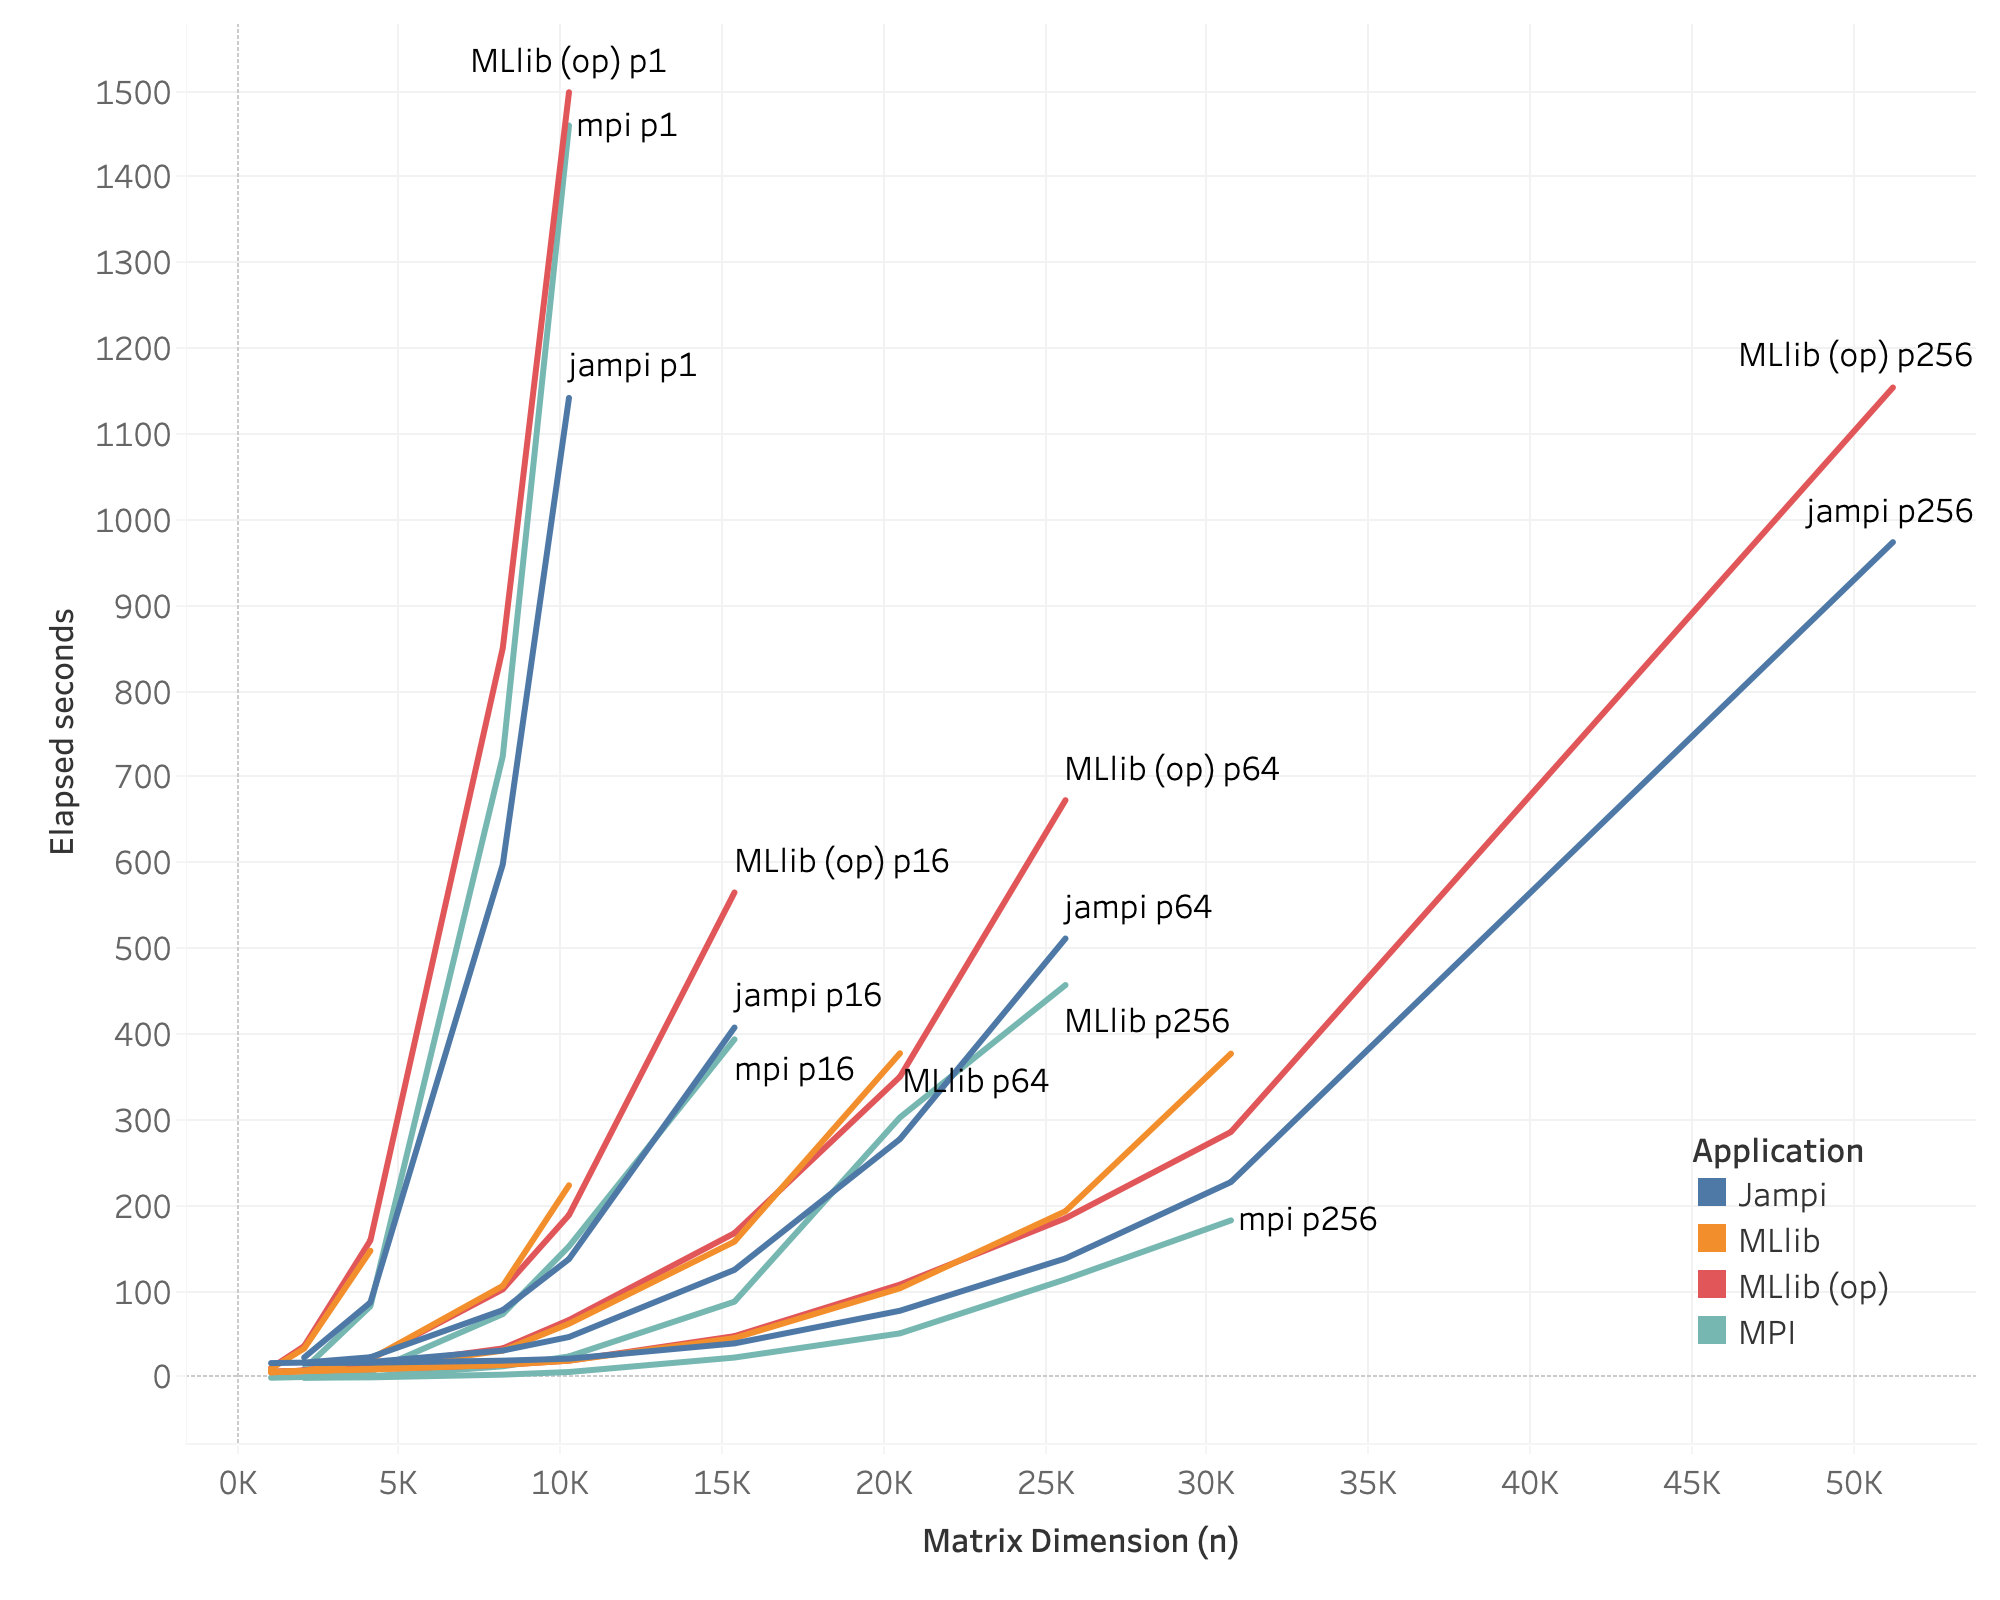
\includegraphics[width=\linewidth]{overall_performance}
\end{figure}

\begin{figure}
	\centering
	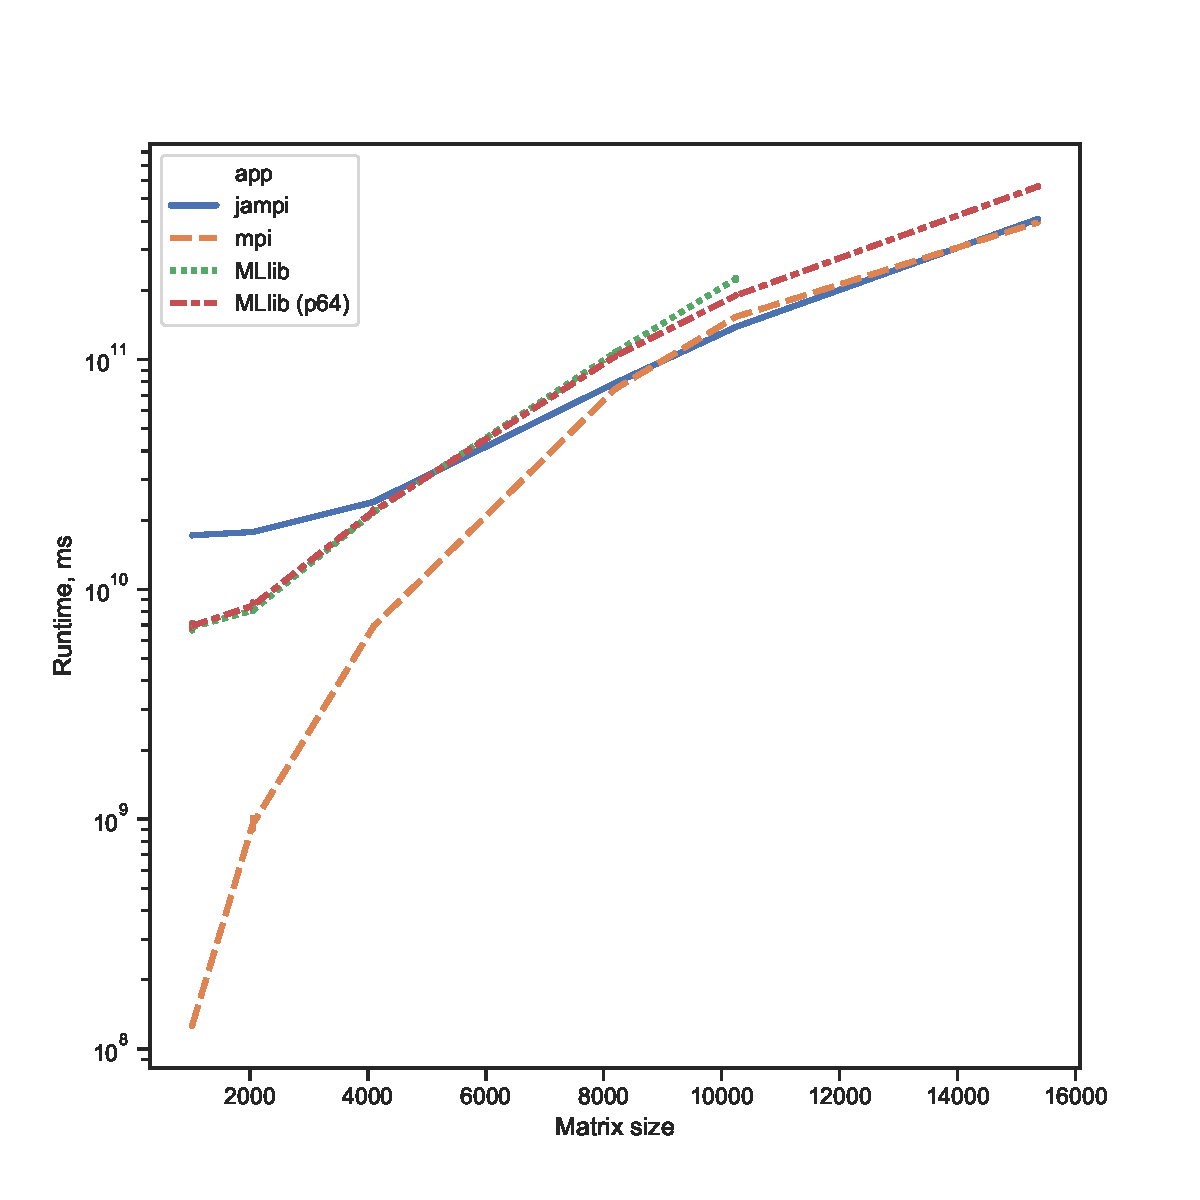
\includegraphics[width=0.9\linewidth]{figures/runtimes.pdf}
	\vspace{14pt}
	\caption{Comparative execution times between JAMPI, MPI, MLlib and MLlib (p64) over $n \times n$ matrices of different sizes.}
	\label{fig:runtimes}
\end{figure}


section

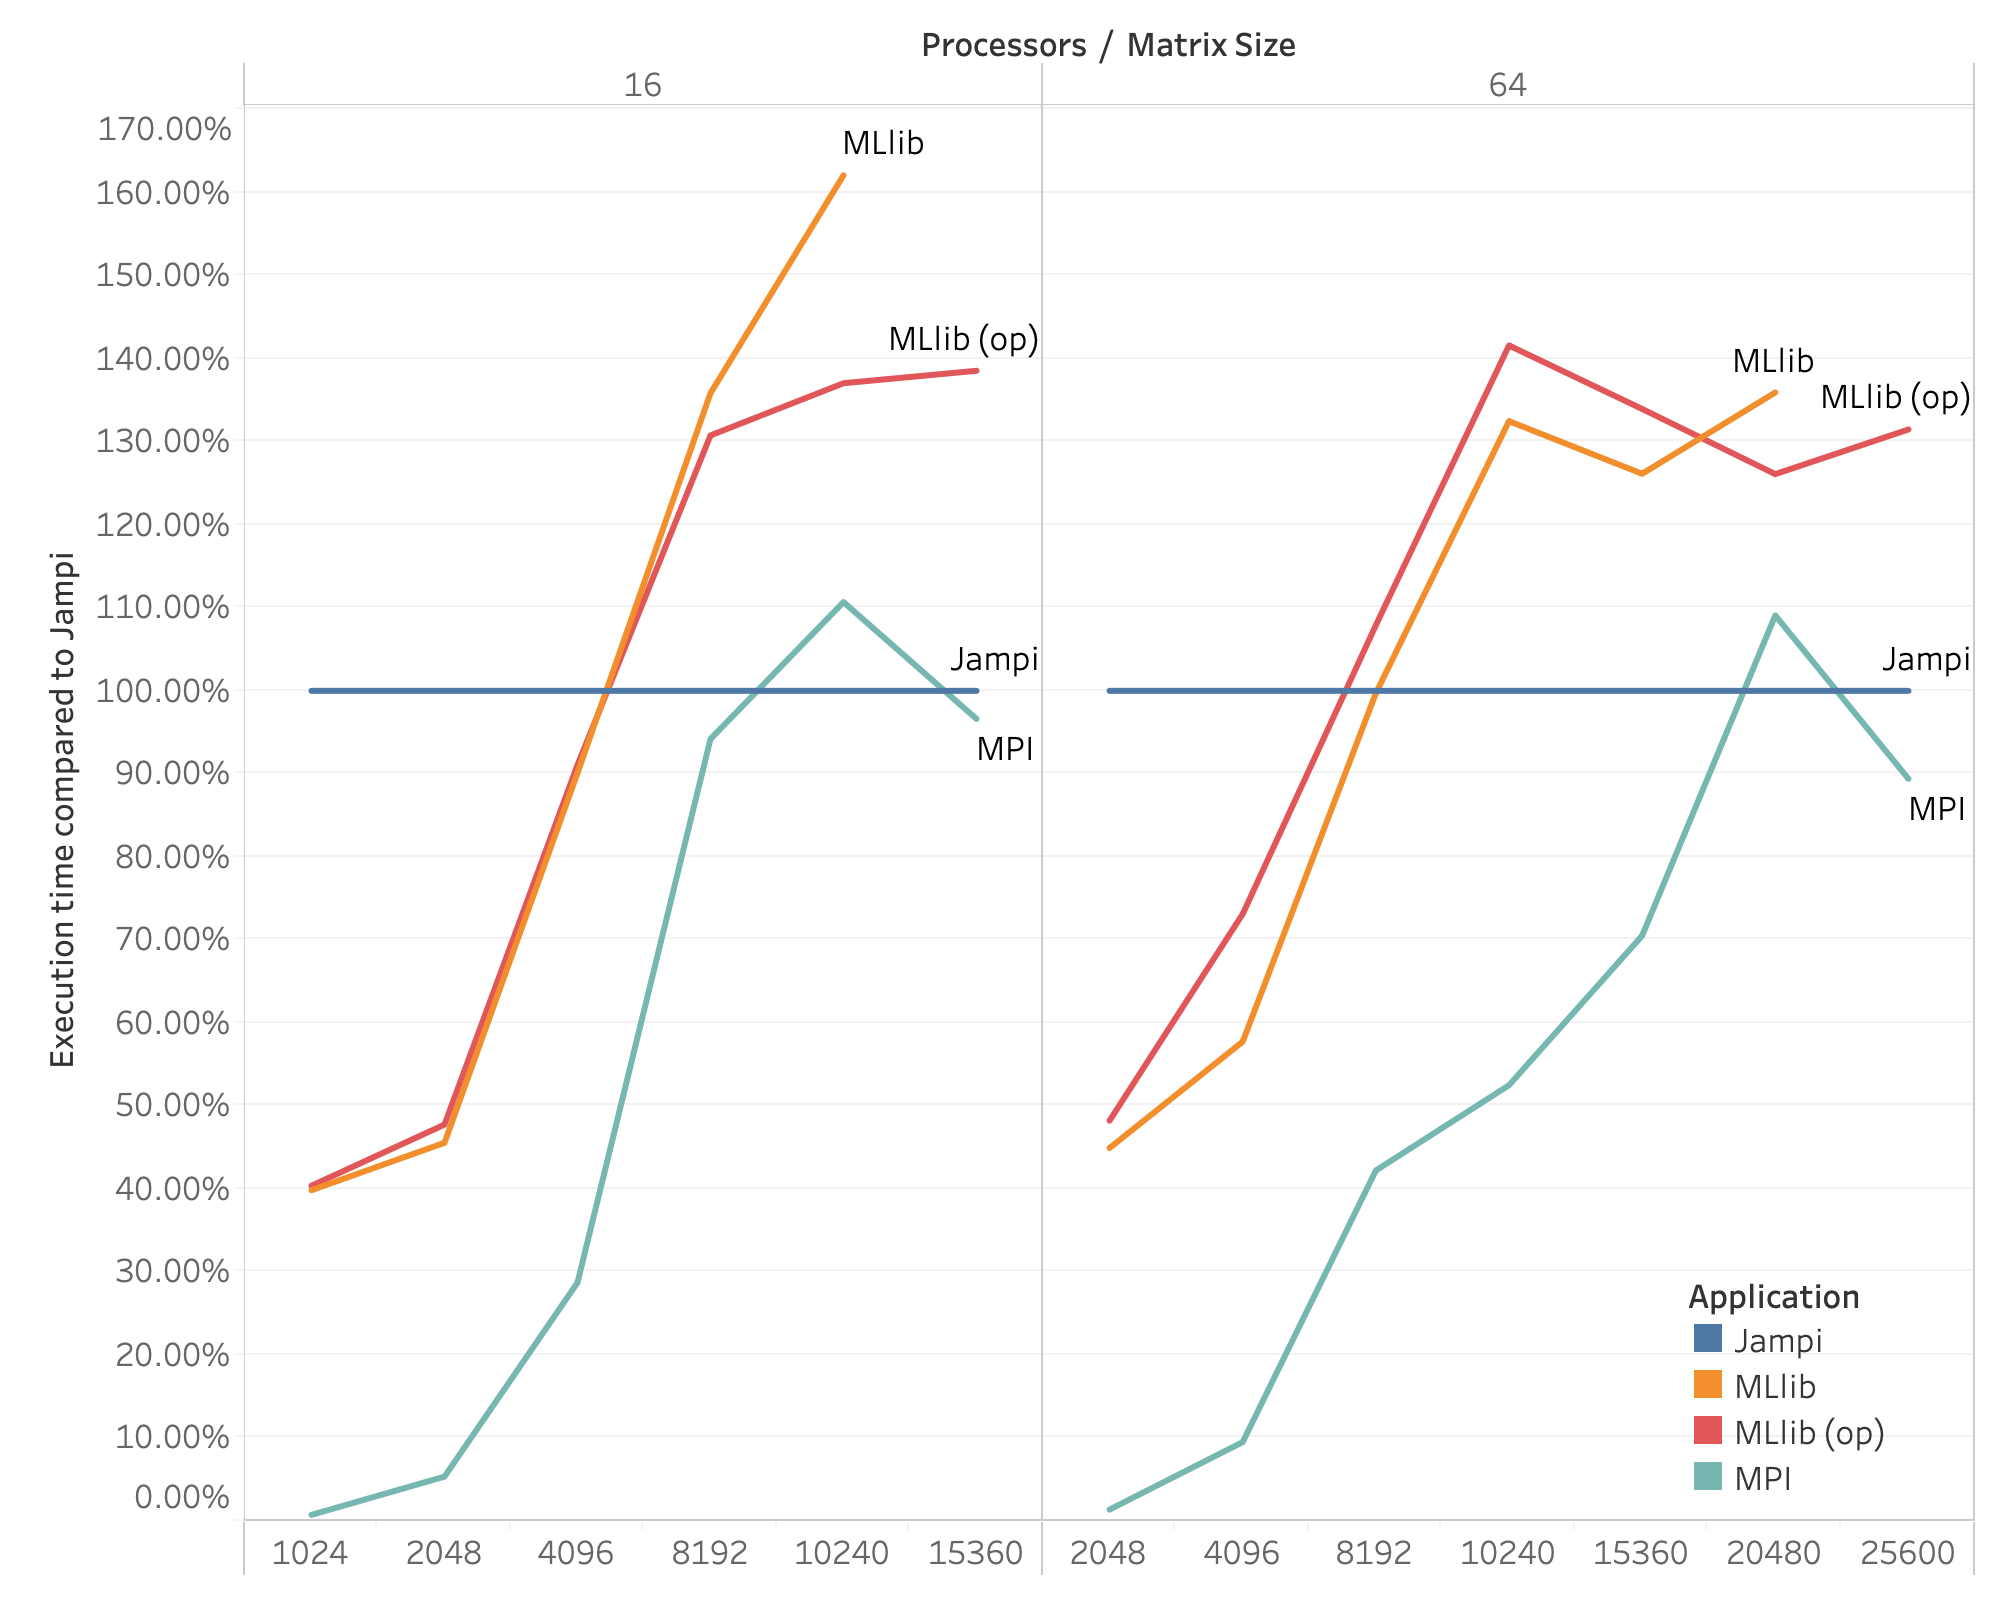
\includegraphics[width=0.9\linewidth]{compared_to_jampi}

Section 


% section results (end)

\section{Conclusion} % (fold)
\label{sec:conclusion}

% section conclusion (end)

%------------------------------------------------
% \phantomsection
% \section*{Acknowledgments} % The \section*{} command stops section numbering

% \addcontentsline{toc}{section}{Acknowledgments} % Adds this section to the table of contents

% All errors and ommissions are the authors' own.

\phantomsection
\section*{Competing interests} % The \section*{} command stops section numbering

% \addcontentsline{toc}{section}{Acknowledgments} % Adds this section to the table of contents

The authors have declared no competing interests.

\phantomsection
\section*{Funding statement} % The \section*{} command stops section numbering

% \addcontentsline{toc}{section}{Acknowledgments} % Adds this section to the table of contents

The research summarised in this paper was funded by Starschema Inc.


%----------------------------------------------------------------------------------------
%	REFERENCE LIST
%----------------------------------------------------------------------------------------
\phantomsection

\bibliographystyle{unsrt}
\bibliography{bibliography}

%----------------------------------------------------------------------------------------

\end{document}
